\section{L'application :}
\textbf{Version minimale Android requise :} Oreo (8.0) (API level 26)

\subsection{Lancement :}
Le projet n'a pas encore été conçu pour être disponible sous un format APK.
\\
Le dépôt git est conçu pour être importé dans Android Studio.
\\
Après avoir cloné le dépôt, rendez vous sur Android Studio puis 
{\textbf {File > New > Import Project}}
et sélectionnez le dossier créé par le clone.

\subsection{Utilisation :}
A l'ouverture de l'application vous obtiendrez l'interface suivante :
\begin{center}
    \begin{minipage}{.48\textwidth}
      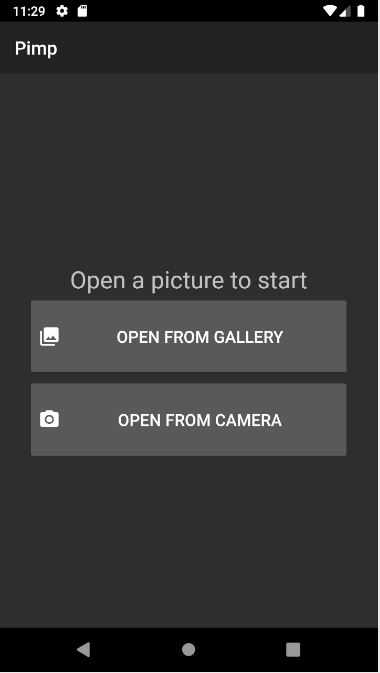
\includegraphics[width=1\textwidth]{report_src/app_manual/first_activity_preview.JPG}
    \end{minipage}
    \begin{minipage}{.48\textwidth}
        Appuyez sur le premier bouton (\faPhoto) pour ouvrir votre galerie photo et choisir une image à importer.
        \\

        Ou appuyez sur le second bouton (\faCamera) pour ouvrir la caméra de votre appareil Android. Capturez alors une image, elle sera sauvegardée dans votre galerie et instantanément importée dans l'application.
        \\

        Il sera nécessaire à la toute première utilisation de ces fonctionnalités d'autoriser l'application à accéder à la galerie et/ou la caméra.
    \end{minipage}
\end{center}
\clearpage

Après avoir choisi une image vous accéderez à la page d'édition principale :
\begin{center}
    \begin{minipage}{.48\textwidth}
      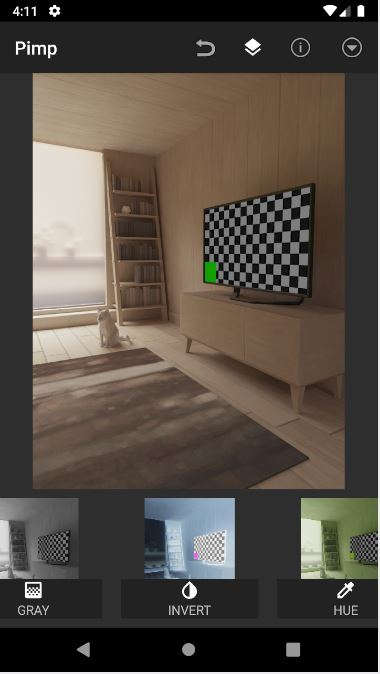
\includegraphics[width=1\textwidth]{report_src/app_manual/main_activity_preview.JPG}
    \end{minipage}
    \begin{minipage}{.48\textwidth}
        Il vous sera possible d'importer une nouvelle image depuis le menu {\faChevronCircleDown}  en haut à droite :
        \begin{center}
        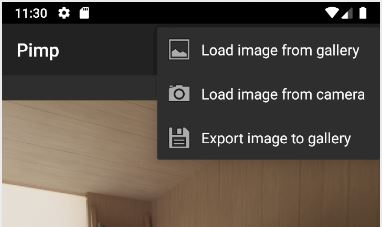
\includegraphics[width=0.8\textwidth]{report_src/app_manual/3dot_button_preview.JPG}
        \end{center}    

        Le bouton {\faSave} permettra d'exporter votre image dans votre galerie, cette opération peut prendre un peu de temps car l'image exportée sera de même taille que l'image d'origine.
        \\

        Vous pouvez manipuler l'image, glissez pour la déplacer et pincez pour zoomer ou dé-zoomer.
    \end{minipage}
\end{center}

En bas de l'écran vous trouverez la liste des effets disponibles applicables sur votre image, faites défiler de droite à gauche.
\\

Le bouton {\faMailReply} annule tout les changements appliqués à l'image en la restaurant à son état d'origine.
\clearpage

Le bouton {\faInfoCircle} quand à lui affiche les informations suivantes à propos de l'image :
\begin{center}
    \begin{minipage}{.48\textwidth}
      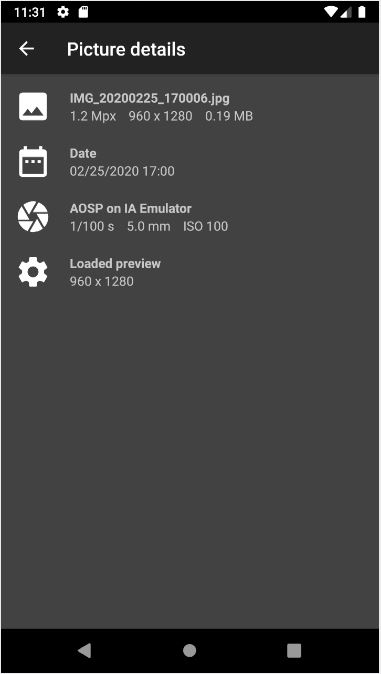
\includegraphics[width=1\textwidth]{report_src/app_manual/info_fragment_preview.JPG}
    \end{minipage}
    \begin{minipage}{.48\textwidth}
        Les sections {\faPhoto} {\faCalendar} {\faChrome} et {\faMapMarker} permettent d'afficher des informations respectivement sur le fichier image, sur sa date de prise de vue, sur l'appareil source et sur ses coordonnées géographiques.
        \\
        Ces sections ne sont pas toujours visibles et dépendent du fichier image.
        \\

        Quand à la section {\faCog} elle donne les dimensions de l'aperçu actuellement affiché dans l'application, il peut être plus petit que l'image d'origine afin de préserver la mémoire du téléphone et le temps d'exécution. L'image exportée en revanche sera aux bonnes dimensions.
    \end{minipage}
\end{center}
\clearpage

Après avoir sélectionné un effet sur la liste en bas de l'écran, des éléments d'interface vont se superposer à votre image :
\begin{center}
    \begin{minipage}{.48\textwidth}
      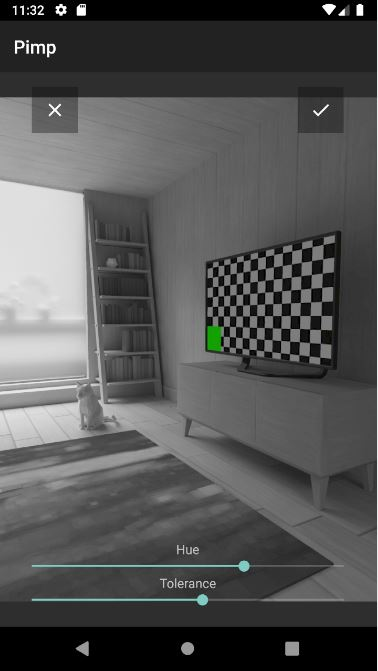
\includegraphics[width=1\textwidth]{report_src/app_manual/effect_fragment_preview.JPG}
    \end{minipage}
    \begin{minipage}{.48\textwidth}
        Le bouton {\faRemove} en haut à gauche vous fait revenir à la liste d'effets et annule l'effet courant.
        \\

        Le bouton {\faCheck} en haut à droite applique l'effet et vous fait revenir à la liste d'effets.
        \\

        En bas des curseurs ou des boutons peuvent apparaître, selon l'effet sélectionné. Manipulez les pour voir en temps réel l'impact sur l'image.
    \end{minipage}
\end{center}

\vspace{2cm}
\textbf{NB:} L'entièreté de cette application est verrouillée en mode portrait.
